%-------------------------------------------------------------------------------
\section{Introduction}
%-------------------------------------------------------------------------------

Application developers increasingly must implement
\emph{privacy transformations} over their applications' data.
%
%Web application developers today have more incentives than ever to provide better privacy for their users.
%
Laws like the EU's General Data Protection Regulation (GDPR)~\cite{eu:gdpr} and California's
Consumer Privacy Act (CCPA)~\cite{ca:privacy-act}
codify the transformations corresponding to some user actions: when a user
closes their account, the site must generally
%
delete “personally identifiable” user data and anonymize or delete other user
contributions.
%
Prudence and good practice recommend other transformations. For example, a
site might scrub or anonymize its older contents to reduce the impact of a
possible later breach, since
%
the legal consequences and reputational damage of breaches can be
substantial~\cite{breach:amazon, breach:twitter, breach:fb, breach:marriott,
breach:quora}.


%
%To write a privacy transformation, developers must carefully map the high-level privacy policy to
%operations that delete or rewrite data objects, while ensuring that the application preserves
%utility for other users, retains legally-mandated anonymized data, and avoids violating application
%invariants.
%
%For example, deleting a user's account should not unexpectedly grant broad access to
%previously-private content by deleting objects that restrict access, nor should it make
%non-sensitive shared content disappear.
%%
%Developers must also consider indirectly identifying correlations between data objects: for example,
%anonymized public running routes can identify the user's hometown and even the
%user~\cite{strava:heatmap}, and anonymized order histories in e-commerce sites can reidentify
%buyers.

\begin{figure}[t]
    \centering
    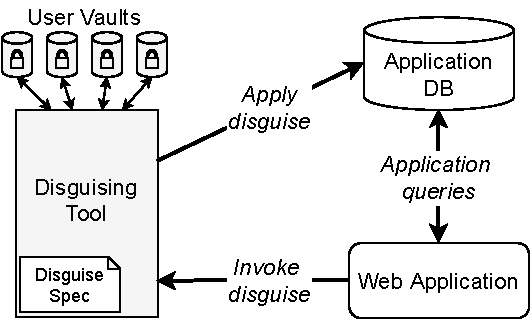
\includegraphics[width=0.35\textwidth]{img/disguise_tool}
    \caption{A data disguising tool takes a developer's disguise specification and transforms
	     a web application's database contents. Per-user vaults
	     (which can be encrypted and stored on third-party storage) support reversible
	     privacy transformations by logging the changes to each user's data.}
    \label{fig:tool}
\end{figure}

%
%The burden of implementing privacy transformations grows with the underlying privacy policy's
%complexity.
%
%Although simplicity has advantages, more nuanced privacy policies are important and useful.
%
%Such policies can help protect users against data correlation attacks; they can give more
%control to individuals by allowing them to choose their own, fine-grained privacy semantics; and
%they may enable new privacy modes such as data that gradually ``decays'' to become less identifiable over time.
%
%Likewise, reversible privacy transformations might strike a sweet
%spot---allowing users to remove identifiable information on demand,
%but accommodating service providers' interest to make it easy for users to return---but
%add significant implementation burden.
%

%
%With more nuanced and reversible privacy transformations, developers face an even greater challenge:
%they must reason about how these privacy transformations compose. For example, an application may
%automatically decay data over time, but must still correctly remove a user's data when they delete
%their account, even if this data has been anonymized.
%Ensuring that one privacy transformation does not affect the privacy properties
%achieved by future transformations, even if they both transform the same data, is a non-trivial task.
%


%Today, developers must manually implement these transformations as part of their application
%code, which is error-prone, laborious, and begets ad-hoc solutions.

%
In this paper, we propose \emph{data disguising}, a systematic framework that helps developers
of database-backed web applications specify, implement, and reason about privacy transformations.
%
Data disguising supports a broad range of privacy transformations and separates the application
of privacy transformations (``data disguises'') from application code.
%
Developers provide disguise specifications to an external disguising tool, which computes the necessary
database changes and applies them to the application's database backend (Figure~\ref{fig:tool}).
%
Applying a disguise transforms the application data to meet a privacy-oriented goal (\eg
deleting users' identifiers, or decorrelating identifying object relationships) while preserving
application invariants and utility.
%
It also can integrate new components, such as \emph{user vaults}, that support new, more nuanced policies than most current applications.


%% \eddie{Lily, do not edit this to make it sound like all disguises have to be reversible.}

\begin{comment}
\lyt{Frans comment: What is the point of this 3rd paragraph?}
Although privacy is often thought of as monotonic---for instance, users can
leave a system, but not return---we believe a more flexible set of privacy
transformations would improve application experience and better meet user
needs.
%
Thus, the data disguising framework can integrate \emph{per-user vaults}, which are
separate, mostly-offline storage shards that log disguises applied to an individual user's data.
%
Vaults allow for selective and partial disguise reversal (\eg when a user
wants to return to the application, or, potentially, to apply another disguise).
%
Vaults cannot be accessed by application queries, and can be deployed in different
ways and with different levels of privacy guarantee.
%
For instance, vaults might be physically co-located with or separate from the the
application storage; encrypted or unencrypted; and access might require explicit
user approval.
%
\end{comment}

%

%
We believe that a systematic, yet flexible approach to disguising addresses applications'
diverse privacy requirements, reduces developer burden, and ultimately achieves better user privacy on
the web.
%
However, our framework is far from complete and realizing it will require solving several research
problems.
%
First, when an application contains more than one privacy transformation, the respective
data disguises may have co-dependencies: for example, removing a user's data on account
deletion is challenging if that data has already been anonymized and decorrelated from the
user.
%
A practical data disguising tool could use a combination of static analysis,
warnings to developers, privacy assertions, and access to possibly-encrypted
vault information to ensure disguises compose correctly.
%
Second, the performance impact of data disguises could be substantial, particularly if they
transform many database rows, and especially if they act on a live application database.
%
We argue that these are important challenges for researchers to investigate to make data
disguising practical.
%
Our proof-of-concept data disguising tool, \sys, demonstrates the potential of this
approach.
%
%Disguises do not guarantee strict privacy---a disguise's content might still expose user
%information or correlated data if not redacted by the policy---but flexible disguising,
%rather than universal deletion, is what real applications require.
%
%Disguises consist of transformations performed on the high-level object graph embedded in
%database-based applications (encoded by \eg foreign key relationships in relational
%databases)~\cite{orms}.
%
%A data disguising tool takes a disguise and its target, and automatically applies the appropriate
%transformations to application data to achieve the disguised state, handling
%disguise composition and disguise interdependencies. Developers can
%thus reason at a high level about each disguise in isolation, reducing the developer burden.
%
%
%\sys proxies relational database operations and exposes APIs to invoke privacy transformations.
%
